\chapter{Результаты}
Для получения более качественных результатов, а также многократоно
сократив время расчетов и исследований, проведем кроссвалидацию
гиперпараметров модели в два этапа. Сперва используем адаптивную
функцию активации REAct \cite{0d752c79fb816703274a3d37f85a85689a2a9405},
в силу ее простоты и скорости вычисления значения и производной, что 
позволяет проводить кроссвалидацию намного эффективнее. Так как теоритически
нельзя предсказать поведение модели при разных параметрах, кроссвалидация
проводится по средствам поиска по сетке. В качестве
гиперпараметров будем итерировать конфигурацию нейронной сети, оптимизатору,
количеству точек внутри области и скорости обучения.

Архитектура нейронной сети исследовалась с вариативным подбором слоёв:
от компактных структур, таких как $16-16$ и $32-32$, до более глубоких
комбинаций --- $32-64-32$, $64-32-64$ и даже асимметричных схем, включающих
$16-32-64$, $64-32-16$, $16-64-32$ и $64-16-32$. Отдельное внимание уделялось
масштабируемым конфигурациям, таким как $64-64$, для оценки влияния
количества нейронов на производительность модели.

Для исследования влияния оптимизатора на результат были выбраны
следующие оптимизаторы: \textbf{Adam}, \textbf{Adagrad}, \textbf{Adamax},
а также специализированные \textbf{ASGD} и \textbf{RMSprop}.

Обучающая выборка варьировалась между $100$ и $500$ точками для внутренней
области и неизменных $1000$ точек для граничных условий. 

Скорость обучения задавалась тремя значениями: $10^{-1}$, $10^{-2}$ и $10^{-3}$.


\begin{figure}[ht]
    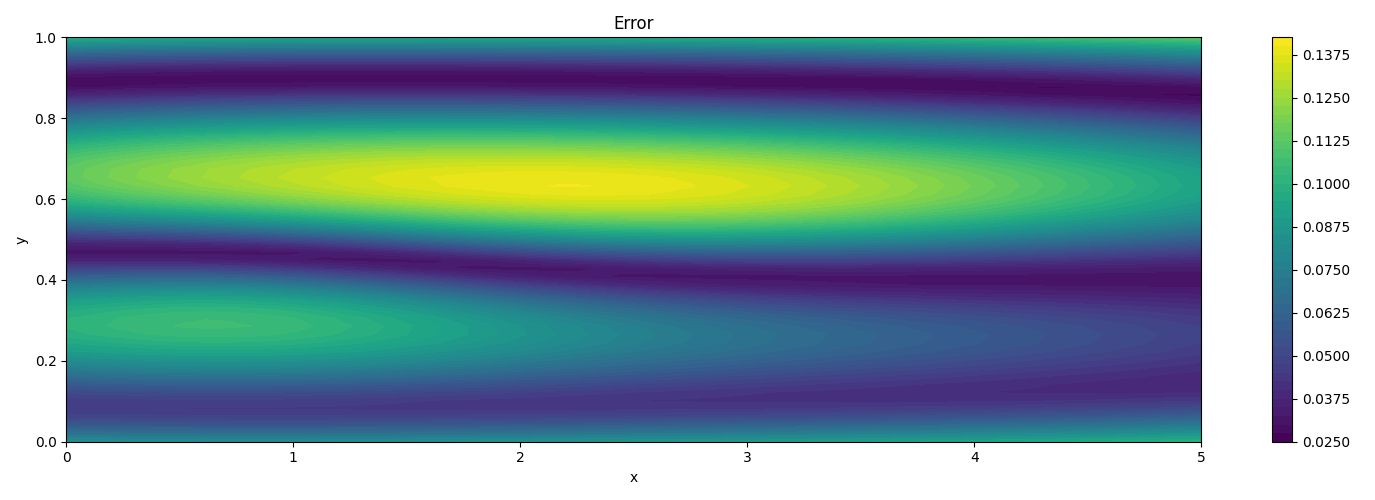
\includegraphics{data/couette_react_error_best.png}
    \caption{Лучший результат в процессе кроссвалидации с функцией активации REAct}
    \label{fig:couette_react_best}
\end{figure}


В результате обучения модель с предсказанным минимальным отклонением от
верного решения (рис. \ref{fig:couette_react_best}) имела следующие значения
гиперпараметров (табл. \ref{table:couette_react_best_params}).

\begin{table}[h!]
    \centering
    \begin{tabular}{ |c|c| } 
        \hline
        Функция активации & $\text{REAct}(0.8, -4, -3.2, 0.2)$ \\
        \hline
        Оптимизатор & Adagrad \\ 
        \hline
        Конфигурация сети & $64-16-32$ \\ 
        \hline
        Скорость обучения & $10^{-3}$ \\ 
        \hline
        Количество точек внутри области & $100$ \\ 
        \hline
    \end{tabular}
    \caption{Значения гиперпараметров у модели с лучшим результатом}
    \label{table:couette_react_best_params}
\end{table}

В результате анализа остальных моделей было посчитано количество нулевых
решений, решений с максимальным отклонением до 20\%, а также больше 20\% и 50\%.
Помимо перечисленных также было несколько моделей, ушедших в процессе обучения в
NaN (рис. \ref{fig:couette_react_stat}). 

\begin{figure}[ht]
    \centering
    \begin{tikzpicture}
        \pgfplotstableread{
        Label   First
        NaN                     4
        Нулевое\ решение        30
        $>50\%$                 16
        $>20\%$                 94
        $<20\%$                 17
        }\datatable
        
        \begin{axis}[
            xbar stacked,
            xmin=0,
            ytick=data,
            yticklabels from table={\datatable}{Label}
            ]
            \addplot [fill=yellow] table [x=First, y expr=\coordindex] {\datatable};
        \end{axis}
    \end{tikzpicture}
    \caption{Распределение результатов кроссвалидации с функцией активации REAct}
    \label{fig:couette_react_stat}
\end{figure}

Также стоит отметить, что все нулевые решения соответствовали функции активации,
которая на всей области определения имеет отрицательные значения.

В качестве корректных параметров были отобраны те, которые соответствуют критерию
принадлежности к группе с уровнем менее 20\%. В результате, во второй этап были
включены следующие параметры:
\begin{enumerate}
    \item Конфигурации с резким переходом между слоями ($16-64-32$ и $64-16-32$) а также
    с линейным переходом ($16-32-64$ и $64-32-16$) не показали особых результатов по
    сравнению с остальными трехслойными сетями. Аналогично конфигурации
    $16-16$ и $32-32$ показали себя хуже по сравнению с $64-64$.
    \item По количеству точек внутри области значительно больше удачных
    результатов было при $100$ точек. Это поведение характеризуется 
    соотношением точек на границе и внутри области. Данное соотношение 
    показывает значимость граничных условий, что необходимо для избегания
    нулевого решения
    \item Скорость обучения влияет на то, сможет ли оптимизатор 
    выбраться из локального минимума. Лучший результат показало значение
    скорости обучения равное $10^{-3}$
    \item Среди оптимизаторов лучшие результаты показали \textbf{Adam}, \textbf{Adagrad} и
    \textbf{ASGD}, в свою очередь \textbf{Adamax} и \textbf{RSMProp} являются узкоспециализированными,
    что требует точной настройки параметров, что в данной работе не рассматривается.
\end{enumerate} 

Теперь получив более точное представление о наших параметрах можно приступить
ко второму этапу обучения с использованием комплексной функцией активации \textbf{ABU} \cite{Sutfeld2018-io}.

Для более корректной оценки результатов будем анализировать медиану для каждого параметра
на протяжении всего этапа обучения.

В представленных ниже графиках показано сравнение результатов работы нейронной сети
при различных гиперпараметрах. Такой подход позволяет детально проанализировать
влияние каждого параметра на общую эффективность модели и выявить, какие параметры
обеспечивают наилучшее качество обучения.
\begin{figure}[ht]
    \centering
    \begin{subfigure}[b]{0.4\textwidth}
        \begin{tikzpicture}
            \begin{axis}[
                ymode=log,
                % xlabel={Эпоха},
                ylabel={Медиана},
                xmin=0,
                xtick distance=4000,
                axis lines=left,
                grid=both,
                title={Нижняя граница},
                width=\textwidth
            ]
            \addplot+[mark=*, mark size=1pt, thick, red] table[x=step, y=value, col sep=comma]{data/couette_abu/loss/bc_bottom_neurons_(32, 64, 32).csv};
            \addplot+[mark=*, mark size=1pt, thick, green] table[x=step, y=value, col sep=comma]{data/couette_abu/loss/bc_bottom_neurons_(64, 32, 64).csv};
            \addplot+[mark=*, mark size=1pt, thick, blue] table[x=step, y=value, col sep=comma]{data/couette_abu/loss/bc_bottom_neurons_(64, 64).csv};
            \addplot+[mark=*, mark size=1pt, thick, orange] table[x=step, y=value, col sep=comma]{data/couette_abu/loss/bc_bottom_neurons_(128, 128).csv};
            \end{axis}
        \end{tikzpicture}
        \label{fig:bc_bottom}
    \end{subfigure}
    \hspace{0.5cm}
    \begin{subfigure}[b]{0.4\textwidth}
        \begin{tikzpicture}
            \begin{axis}[
                ymode=log,
                % xlabel={Эпоха},
                % ylabel={Медиана},
                xmin=0,
                xtick distance=4000,
                axis lines=left,
                grid=both,
                title={Верхняя граница},
                width=\textwidth
            ]
            \addplot+[mark=*, mark size=1pt, thick, red] table[x=step, y=value, col sep=comma]{data/couette_abu/loss/bc_top_neurons_(32, 64, 32).csv};
            \addplot+[mark=*, mark size=1pt, thick, green] table[x=step, y=value, col sep=comma]{data/couette_abu/loss/bc_top_neurons_(64, 32, 64).csv};
            \addplot+[mark=*, mark size=1pt, thick, blue] table[x=step, y=value, col sep=comma]{data/couette_abu/loss/bc_top_neurons_(64, 64).csv};
            \addplot+[mark=*, mark size=1pt, thick, orange] table[x=step, y=value, col sep=comma]{data/couette_abu/loss/bc_top_neurons_(128, 128).csv};
            \end{axis}
        \end{tikzpicture}
        \label{fig:bc_top}
    \end{subfigure}
    \vspace{0.05cm}
    \begin{subfigure}[b]{0.4\textwidth}
        \begin{tikzpicture}
            \begin{axis}[
                ymode=log,
                xlabel={Эпоха},
                ylabel={Медиана},
                xmin=0,
                xtick distance=4000,
                axis lines=left,
                grid=both,
                title={Левая граница},
                width=\textwidth
            ]
            \addplot+[mark=*, mark size=1pt, thick, red] table[x=step, y=value, col sep=comma]{data/couette_abu/loss/bc_left_neurons_(32, 64, 32).csv};
            \addplot+[mark=*, mark size=1pt, thick, green] table[x=step, y=value, col sep=comma]{data/couette_abu/loss/bc_left_neurons_(64, 32, 64).csv};
            \addplot+[mark=*, mark size=1pt, thick, blue] table[x=step, y=value, col sep=comma]{data/couette_abu/loss/bc_left_neurons_(64, 64).csv};
            \addplot+[mark=*, mark size=1pt, thick, orange] table[x=step, y=value, col sep=comma]{data/couette_abu/loss/bc_left_neurons_(128, 128).csv};
            \end{axis}
        \end{tikzpicture}
        \label{fig:bc_left}
    \end{subfigure}
    \hspace{0.5cm}
    \begin{subfigure}[b]{0.4\textwidth}
        \begin{tikzpicture}
            \begin{axis}[
                ymode=log,
                xlabel={Эпоха},
                % ylabel={Медиана},
                xmin=0,
                xtick distance=4000,
                axis lines=left,
                grid=both,
                title={Правая граница},
                width=\textwidth
            ]
            \addplot+[mark=*, mark size=1pt, thick, red] table[x=step, y=value, col sep=comma]{data/couette_abu/loss/bc_right_neurons_(32, 64, 32).csv};
            \addplot+[mark=*, mark size=1pt, thick, green] table[x=step, y=value, col sep=comma]{data/couette_abu/loss/bc_right_neurons_(64, 32, 64).csv};
            \addplot+[mark=*, mark size=1pt, thick, blue] table[x=step, y=value, col sep=comma]{data/couette_abu/loss/bc_right_neurons_(64, 64).csv};
            \addplot+[mark=*, mark size=1pt, thick, orange] table[x=step, y=value, col sep=comma]{data/couette_abu/loss/bc_right_neurons_(128, 128).csv};
            \end{axis}
        \end{tikzpicture}
        \label{fig:bc_right}
    \end{subfigure}
    \caption{Зависимость медианы функции потерь на каждой эпохе при разной конфигурации нейронной сети}
    \label{fig:bc_loss_neurons}
\end{figure}

%%%%%%%%%%%%%%%%%%%%%%%%%%%%%%%%%%%%%%%%%%%%%%%%%%%%%%%%%%%%%%%%%%%%%%%%%%%%%%

\begin{figure}[htbp]
    \centering
    \begin{subfigure}[b]{0.4\textwidth}
        \begin{tikzpicture}
            \begin{axis}[
                ymode=log,
                ymin=1e-4, ymax=1e-2,
                xlabel={Эпоха},
                ylabel={Медиана},
                xmin=0,
                xtick distance=4000,
                axis lines=left,
                grid=both,
                title={Уравнение для $v_x$},
                width=\textwidth
            ]
            \addplot+[mark=*, mark size=1pt, thick, red] table[x=step, y=value, col sep=comma]{data/couette_abu/loss/pde_momentum_x_neurons_(32, 64, 32).csv};
            \addplot+[mark=*, mark size=1pt, thick, green] table[x=step, y=value, col sep=comma]{data/couette_abu/loss/pde_momentum_x_neurons_(64, 32, 64).csv};
            \addplot+[mark=*, mark size=1pt, thick, blue] table[x=step, y=value, col sep=comma]{data/couette_abu/loss/pde_momentum_x_neurons_(64, 64).csv};
            \addplot+[mark=*, mark size=1pt, thick, orange] table[x=step, y=value, col sep=comma]{data/couette_abu/loss/pde_momentum_x_neurons_(128, 128).csv};
            \end{axis}
        \end{tikzpicture}
    \end{subfigure}
    \hspace{0.5cm}
    \begin{subfigure}[b]{0.4\textwidth}
        \begin{tikzpicture}
            \begin{axis}[
                ymode=log,
                ymin=1e-4, ymax=1e-2,
                xlabel={Эпоха},
                % ylabel={Медиана},
                xmin=0,
                xtick distance=4000,
                axis lines=left,
                grid=both,
                title={Уравнение для $v_y$},
                width=\textwidth
            ]
            \addplot+[mark=*, mark size=1pt, thick, red] table[x=step, y=value, col sep=comma]{data/couette_abu/loss/pde_momentum_y_neurons_(32, 64, 32).csv};
            \addplot+[mark=*, mark size=1pt, thick, green] table[x=step, y=value, col sep=comma]{data/couette_abu/loss/pde_momentum_y_neurons_(64, 32, 64).csv};
            \addplot+[mark=*, mark size=1pt, thick, blue] table[x=step, y=value, col sep=comma]{data/couette_abu/loss/pde_momentum_y_neurons_(64, 64).csv};
            \addplot+[mark=*, mark size=1pt, thick, orange] table[x=step, y=value, col sep=comma]{data/couette_abu/loss/pde_momentum_y_neurons_(128, 128).csv};
            \end{axis}
        \end{tikzpicture}
    \end{subfigure}
    \begin{subfigure}[b]{0.7\textwidth}
        \begin{tikzpicture}
            \begin{axis}[
                ymode=log,
                ymin=1e-4, ymax=1e-2,
                xlabel={Эпоха},
                ylabel={Медиана},
                xmin=0,
                xtick distance=1000,
                axis lines=left,
                grid=both,
                title={Уравнение непрерывности},
                width=\textwidth
            ]
            \addplot+[mark=*, mark size=1pt, thick, red] table[x=step, y=value, col sep=comma]{data/couette_abu/loss/pde_continuity_neurons_(32, 64, 32).csv};
            % \addlegendentry{(32, 64, 32)}
            \addplot+[mark=*, mark size=1pt, thick, green] table[x=step, y=value, col sep=comma]{data/couette_abu/loss/pde_continuity_neurons_(64, 32, 64).csv};
            % \addlegendentry{(64, 32, 64)}
            \addplot+[mark=*, mark size=1pt, thick, blue] table[x=step, y=value, col sep=comma]{data/couette_abu/loss/pde_continuity_neurons_(64, 64).csv};
            % \addlegendentry{(64, 64)}
            \addplot+[mark=*, mark size=1pt, thick, orange] table[x=step, y=value, col sep=comma]{data/couette_abu/loss/pde_continuity_neurons_(128, 128).csv};
            % \addlegendentry{(128, 128)}
        \end{axis}
        \end{tikzpicture}
    \end{subfigure}
    \caption{Функция потерь для уравнений Навье-Стокса \eqref{eq:navier_stockes} при разной конфигурации нейронной сети}
    \label{fig:pde_loss_neurons}
\end{figure}

%%%%%%%%%%%%%%%%%%%%%%%%%%%%%%%%%%%%%%%%%%%%%%%%%%%%%%%%%%%%%%%%%%

\begin{figure}[htbp]
    \centering
    \begin{tikzpicture}
        \begin{axis}[
            width=0.8\textwidth,
            ymode=log,
            xlabel={Эпоха},
            ylabel={Медиана},
            xmin=0,
            xtick distance=1000,
            axis lines=left,
            grid=both,
        ]
            \addplot+[mark=*, mark size=1pt, thick, red] table[x=step, y=value, col sep=comma]{data/couette_abu/loss/total_loss_neurons_(32, 64, 32).csv};
            \addlegendentry{(32, 64, 32)}
            \addplot+[mark=*, mark size=1pt, thick, green] table[x=step, y=value, col sep=comma]{data/couette_abu/loss/total_loss_neurons_(64, 32, 64).csv};
            \addlegendentry{(64, 32, 64)}
            \addplot+[mark=*, mark size=1pt, thick, blue] table[x=step, y=value, col sep=comma]{data/couette_abu/loss/total_loss_neurons_(64, 64).csv};
            \addlegendentry{(64, 64)}
            \addplot+[mark=*, mark size=1pt, thick, orange] table[x=step, y=value, col sep=comma]{data/couette_abu/loss/total_loss_neurons_(128, 128).csv};
            \addlegendentry{(128, 128)}
        \end{axis}
    \end{tikzpicture}
    \caption{Итоговая функция потерь при разной конфигурации нейронной сети}
    \label{fig:total_loss_neurons}
\end{figure}
\section{Зависимость от оптимизатора}

С точки зрения оптимизатора никаких ограничений на поведение
модели нет. От выбора оптимизатора зависит на сколько сложно
модели будет выбраться из локального минимума и приблизиться
к глобальному.

Рассмотрим верхнюю границу (рис \ref{fig:bc_top_optimizer}).
Исходя из графика, при использовании оптимизатора ASGD
функция потерь в среднем стремится к $~0.25$. При такой 
функции потерь максимальное отклонение от точного решения
может достигать $50\%$, если не учитывать полностью
нулевые решения. Сам по себе ASGD является мощным оптимизатором,
но требует тонкой настройки своих параметров, поэтому он
показывает худший результат в данной задаче.

Похожая ситуация с Adagrad оптимизатором, без качественной
настройки параметров скорость обучения адаптивно уменьшается
и оптимизатор застывает в локальном минимуме. Вероятнее всего
при большем числе эпох Adagrad сможет догнать Adam, но нас
данный вариант не устраивает.

Оптимизатор Adam показывает лучший результат. Данный оптимизатор
включает в себя преймущества двух предыдущих и является универсальным,
поэтому не требует такой же точной настройки параметров.

\begin{figure}[ht]
    \centering
    \begin{subfigure}[b]{0.4\textwidth}
        \begin{tikzpicture}[scale=0.85]
            \begin{axis}[
                ymode=log,
                legend style={font=\tiny},
                xmin=0,
                xtick distance=4000,
                axis lines=left,
                grid=both
            ]            
                \addplot+[mark=*, mark size=1pt, thick, red] table[x=step, y=value, col sep=comma]{data/couette_abu/loss/bc_bottom_optimizer_1.csv};
                \addlegendentry{Adam}
                \addplot+[mark=*, mark size=1pt, thick, green] table[x=step, y=value, col sep=comma]{data/couette_abu/loss/bc_bottom_optimizer_2.csv};
                \addlegendentry{Adagrad}
                \addplot+[mark=*, mark size=1pt, thick, blue] table[x=step, y=value, col sep=comma]{data/couette_abu/loss/bc_bottom_optimizer_4.csv};
                \addlegendentry{ASGD}
            \end{axis}
        \end{tikzpicture}
        \caption{Нижняя граница}
        \label{fig:bc_bottom_optimizer}
    \end{subfigure}
    \hspace{0.5cm}
    \begin{subfigure}[b]{0.4\textwidth}
        \begin{tikzpicture}[scale=0.85]
            \begin{axis}[
                ymode=log,
                legend style={font=\tiny},
                xmin=0,
                xtick distance=4000,
                axis lines=left,
                grid=both
            ]
                \addplot+[mark=*, mark size=1pt, thick, red] table[x=step, y=value, col sep=comma]{data/couette_abu/loss/bc_top_optimizer_1.csv};
                \addlegendentry{Adam}
                \addplot+[mark=*, mark size=1pt, thick, green] table[x=step, y=value, col sep=comma]{data/couette_abu/loss/bc_top_optimizer_2.csv};
                \addlegendentry{Adagrad}
                \addplot+[mark=*, mark size=1pt, thick, blue] table[x=step, y=value, col sep=comma]{data/couette_abu/loss/bc_top_optimizer_4.csv};
                \addlegendentry{ASGD}
            \end{axis}
        \end{tikzpicture}
        \caption{Верхняя граница}
        \label{fig:bc_top_optimizer}
    \end{subfigure}
    \begin{subfigure}[b]{0.4\textwidth}
        \begin{tikzpicture}[scale=0.85]
            \begin{axis}[
                ymode=log,
                legend style={font=\tiny},
                xmin=0,
                xtick distance=4000,
                axis lines=left,
                grid=both
            ]
                \addplot+[mark=*, mark size=1pt, thick, red] table[x=step, y=value, col sep=comma]{data/couette_abu/loss/bc_left_optimizer_1.csv};
                \addlegendentry{Adam}
                \addplot+[mark=*, mark size=1pt, thick, green] table[x=step, y=value, col sep=comma]{data/couette_abu/loss/bc_left_optimizer_2.csv};
                \addlegendentry{Adagrad}
                \addplot+[mark=*, mark size=1pt, thick, blue] table[x=step, y=value, col sep=comma]{data/couette_abu/loss/bc_left_optimizer_4.csv};
                \addlegendentry{ASGD}
            \end{axis}
        \end{tikzpicture}
        \caption{Левая граница}
        \label{fig:bc_left_optimizer}
    \end{subfigure}
    \hspace{0.5cm}
    \begin{subfigure}[b]{0.4\textwidth}
        \begin{tikzpicture}[scale=0.85]
            \begin{axis}[
                ymode=log,
                legend style={font=\tiny},
                xmin=0,
                xtick distance=4000,
                axis lines=left,
                grid=both
            ]
                \addplot+[mark=*, mark size=1pt, thick, red] table[x=step, y=value, col sep=comma]{data/couette_abu/loss/bc_right_optimizer_1.csv};
                \addlegendentry{Adam}
                \addplot+[mark=*, mark size=1pt, thick, green] table[x=step, y=value, col sep=comma]{data/couette_abu/loss/bc_right_optimizer_2.csv};
                \addlegendentry{Adagrad}
                \addplot+[mark=*, mark size=1pt, thick, blue] table[x=step, y=value, col sep=comma]{data/couette_abu/loss/bc_right_optimizer_4.csv};
                \addlegendentry{ASGD}
            \end{axis}
        \end{tikzpicture}
        \caption{Правая граница}
        \label{fig:bc_right_optimizer}
    \end{subfigure}
    \caption{Зависимость медианы функции потерь на каждой эпохе при разных оптимизаторах}
    \label{fig:bc_loss_optimizer}
\end{figure}

Аналогичное поведение оптимизаторов можно заметить на графике для нижней
границы (рис. \ref{fig:bc_bottom_optimizer}). На графиках левой
(рис. \ref{fig:bc_left_optimizer}) и правой (рис. \ref{fig:bc_right_optimizer})
границах можно заметить смещение оптимизатора ASGD ближе к Adagrad, что может
свидетельствовать о преобладающем нулевом решении.

%%%%%%%%%%%%%%%%%%%%%%%%%%%%%%%%%%%%%%%%%%%%%%%%%%%%%%%%%%%%%%%%%%%%%%%%%%%%%%

\begin{figure}[htbp]
    \centering
    \begin{subfigure}[b]{0.4\textwidth}
        \centering
        \begin{tikzpicture}[scale=0.85]
            \begin{axis}[
                ymode=log,
                ymax=1e-2,
                legend style={font=\tiny},
                xmin=0,
                xtick distance=4000,
                axis lines=left,
                grid=both
            ]
                \addplot+[mark=*, mark size=1pt, thick, red] table[x=step, y=value, col sep=comma]{data/couette_abu/loss/pde_momentum_x_optimizer_1.csv};
                \addlegendentry{Adam}
                \addplot+[mark=*, mark size=1pt, thick, green] table[x=step, y=value, col sep=comma]{data/couette_abu/loss/pde_momentum_x_optimizer_2.csv};
                \addlegendentry{Adagrad}
                \addplot+[mark=*, mark size=1pt, thick, blue] table[x=step, y=value, col sep=comma]{data/couette_abu/loss/pde_momentum_x_optimizer_4.csv};
                \addlegendentry{ASGD}
            \end{axis}
        \end{tikzpicture}
        \caption{Уравнение для $u_x$}
        \label{fig:pde_ux_optimizer}
    \end{subfigure}
    \hspace{0.5cm}
    \begin{subfigure}[b]{0.4\textwidth}
        \centering
        \begin{tikzpicture}[scale=0.85]
            \begin{axis}[
                ymode=log,
                ymax=1e-2,
                legend style={font=\tiny},
                xmin=0,
                xtick distance=4000,
                axis lines=left,
                grid=both
            ]
                \addplot+[mark=*, mark size=1pt, thick, red] table[x=step, y=value, col sep=comma]{data/couette_abu/loss/pde_momentum_y_optimizer_1.csv};
                \addlegendentry{Adam}
                \addplot+[mark=*, mark size=1pt, thick, green] table[x=step, y=value, col sep=comma]{data/couette_abu/loss/pde_momentum_y_optimizer_2.csv};
                \addlegendentry{Adagrad}
                \addplot+[mark=*, mark size=1pt, thick, blue] table[x=step, y=value, col sep=comma]{data/couette_abu/loss/pde_momentum_y_optimizer_4.csv};
                \addlegendentry{ASGD}
            \end{axis}
        \end{tikzpicture}
        \caption{Уравнение для $u_y$}
        \label{fig:pde_uy_optimizer}
    \end{subfigure}
    \begin{subfigure}[b]{0.7\textwidth}
        \centering
        \begin{tikzpicture}
            \begin{axis}[
                ymode=log,
                ymax=1e-2,
                legend style={font=\small},
                xmin=0,
                xtick distance=1000,
                axis lines=left,
                grid=both,
                width=\textwidth
            ]
                \addplot+[mark=*, mark size=1pt, thick, red] table[x=step, y=value, col sep=comma]{data/couette_abu/loss/pde_continuity_optimizer_1.csv};
                \addlegendentry{Adam}
                \addplot+[mark=*, mark size=1pt, thick, green] table[x=step, y=value, col sep=comma]{data/couette_abu/loss/pde_continuity_optimizer_2.csv};
                \addlegendentry{Adagrad}
                \addplot+[mark=*, mark size=1pt, thick, blue] table[x=step, y=value, col sep=comma]{data/couette_abu/loss/pde_continuity_optimizer_4.csv};
                \addlegendentry{ASGD}
            \end{axis}
        \end{tikzpicture}
        \caption{Уравнение непрерывности}
        \label{fig:pde_continuity_optimizer}
    \end{subfigure}
    \caption{Функция потерь для уравнений Навье-Стокса \eqref{eq:navier_stockes} при разных оптимизаторах}
    \label{fig:pde_loss_optimizer}
\end{figure}

Для уравнений Навье-Стокса можно заметить рост функции потерь для оптимизатора
ASGD (рис. \ref{fig:pde_ux_optimizer} и \ref{fig:pde_continuity_optimizer}).
Таким образом происходит процесс поиска глобального минимума. Дело в том,
что функция потерь для верхней границы много больше, чем для уравнений Навье-Стокса
($10^{-0.8}$ против $10^{-2.9}$). Оптимизатор пытается выбраться из локального 
минимума, где решение стремится к нулевому в силу своей корректности с точки
зрения уравнений Навье-Стокса. Что касательно уравнения для скорости $u_y$
(рис. \ref{fig:pde_uy_optimizer}), график оптимизатора ASGD остается
практически неизменным, что опять же соответствует нулевому решению.
Остальные оптимизаторы имеют поведение схожее с поведением на границах.


%%%%%%%%%%%%%%%%%%%%%%%%%%%%%%%%%%%%%%%%%%%%%%%%%%%%%%%%%%%%%%%%%%

\begin{figure}[htbp]
    \centering
    \begin{tikzpicture}
        \begin{axis}[
            width=0.8\textwidth,
            ymode=log,
            xmin=0,
            xtick distance=1000,
            axis lines=left,
            grid=both,
        ]
            \addplot+[mark=*, mark size=1pt, thick, red] table[x=step, y=value, col sep=comma]{data/couette_abu/loss/total_loss_optimizer_1.csv};
            \addlegendentry{Adam}
            \addplot+[mark=*, mark size=1pt, thick, green] table[x=step, y=value, col sep=comma]{data/couette_abu/loss/total_loss_optimizer_2.csv};
            \addlegendentry{Adagrad}
            \addplot+[mark=*, mark size=1pt, thick, blue] table[x=step, y=value, col sep=comma]{data/couette_abu/loss/total_loss_optimizer_4.csv};
            \addlegendentry{ASGD}
        \end{axis}
    \end{tikzpicture}
    \caption{Итоговая функция потерь при разных оптимизаторах}
    \label{fig:total_loss_optimizer}
\end{figure}

Итого на суммарной функции потерь (рис. \ref{fig:total_loss_optimizer}),
оптимизатор Adam имеет наименьшую функцию потерь.
\section{Зависимость от фукции активации ABU}

В первую очередь функция активация играет основополагающую роль для
детерминирования поведения внутри домена. Это связано с тем, что
уравнения Навье-Стокса имеют сложную структуру. Если поставленная
задача имеет не нулевое решение, то нахождение верного решения внутри
домена зависит только от функции активации. Это означает, что нет смысла
ориентироваться на функцию потерь на границах.

Как ранее упоминалось, ABU является взвешенной суммой элементарных функций
активации. Рассмотрим влияние каждого слагаемого на функцию потерь.
\subsection{Квадратичная функция}
\begin{figure}[ht]
    \centering
    \begin{subfigure}[b]{0.4\textwidth}
        \begin{tikzpicture}[scale=0.85]
            \begin{axis}[
                ymode=log,
                legend style={font=\tiny},
                xmin=0,
                xtick distance=4000,
                axis lines=left,
                grid=both
            ]            
                \addplot+[mark=*, mark size=1pt, thick, red] table[x=step, y=value, col sep=comma]{data/couette_abu/loss/bc_bottom_scale_quadratic_0.0.csv};
                \addlegendentry{$0.0$}
                \addplot+[mark=*, mark size=1pt, thick, green] table[x=step, y=value, col sep=comma]{data/couette_abu/loss/bc_bottom_scale_quadratic_1.0.csv};
                \addlegendentry{$1.0$}
            \end{axis}
        \end{tikzpicture}
        \caption{Нижняя граница}
        \label{fig:bc_bottom_scale_quadratic}
    \end{subfigure}
    \hspace{0.5cm}
    \begin{subfigure}[b]{0.4\textwidth}
        \begin{tikzpicture}[scale=0.85]
            \begin{axis}[
                ymode=log,
                legend style={font=\tiny},
                xmin=0,
                xtick distance=4000,
                axis lines=left,
                grid=both
            ]
                \addplot+[mark=*, mark size=1pt, thick, red] table[x=step, y=value, col sep=comma]{data/couette_abu/loss/bc_top_scale_quadratic_0.0.csv};
                \addlegendentry{$0.0$}
                \addplot+[mark=*, mark size=1pt, thick, green] table[x=step, y=value, col sep=comma]{data/couette_abu/loss/bc_top_scale_quadratic_1.0.csv};
                \addlegendentry{$1.0$}
            \end{axis}
        \end{tikzpicture}
        \caption{Верхняя граница}
        \label{fig:bc_top_scale_quadratic}
    \end{subfigure}
    \begin{subfigure}[b]{0.4\textwidth}
        \begin{tikzpicture}[scale=0.85]
            \begin{axis}[
                ymode=log,
                legend style={font=\tiny},
                xmin=0,
                xtick distance=4000,
                axis lines=left,
                grid=both
            ]
                \addplot+[mark=*, mark size=1pt, thick, red] table[x=step, y=value, col sep=comma]{data/couette_abu/loss/bc_left_scale_quadratic_0.0.csv};
                \addlegendentry{$0.0$}
                \addplot+[mark=*, mark size=1pt, thick, green] table[x=step, y=value, col sep=comma]{data/couette_abu/loss/bc_left_scale_quadratic_1.0.csv};
                \addlegendentry{$1.0$}
            \end{axis}
        \end{tikzpicture}
        \caption{Левая граница}
        \label{fig:bc_left_scale_quadratic}
    \end{subfigure}
    \hspace{0.5cm}
    \begin{subfigure}[b]{0.4\textwidth}
        \begin{tikzpicture}[scale=0.85]
            \begin{axis}[
                ymode=log,
                legend style={font=\tiny},
                xmin=0,
                xtick distance=4000,
                axis lines=left,
                grid=both
            ]
                \addplot+[mark=*, mark size=1pt, thick, red] table[x=step, y=value, col sep=comma]{data/couette_abu/loss/bc_right_scale_quadratic_0.0.csv};
                \addlegendentry{$0.0$}
                \addplot+[mark=*, mark size=1pt, thick, green] table[x=step, y=value, col sep=comma]{data/couette_abu/loss/bc_right_scale_quadratic_1.0.csv};
                \addlegendentry{$1.0$}
            \end{axis}
        \end{tikzpicture}
        \caption{Правая граница}
        \label{fig:bc_right_scale_quadratic}
    \end{subfigure}
    \caption{Зависимость медианы функции потерь на каждой эпохе при разных коэффициентов для функции активации Quadratic}
    \label{fig:bc_loss_scale_quadratic}
\end{figure}

Аналогичное поведение оптимизаторов можно заметить на графике для нижней
границы (рис. \ref{fig:bc_bottom_scale_quadratic}). На графиках левой
(рис. \ref{fig:bc_left_scale_quadratic}) и правой (рис. \ref{fig:bc_right_scale_quadratic})
границах можно заметить смещение оптимизатора ASGD ближе к Adagrad, что может
свидетельствовать о преобладающем нулевом решении.

%%%%%%%%%%%%%%%%%%%%%%%%%%%%%%%%%%%%%%%%%%%%%%%%%%%%%%%%%%%%%%%%%%%%%%%%%%%%%%

\begin{figure}[htbp]
    \centering
    \begin{subfigure}[b]{0.4\textwidth}
        \centering
        \begin{tikzpicture}[scale=0.85]
            \begin{axis}[
                ymode=log,
                ymax=1e-2,
                legend style={font=\tiny},
                xmin=0,
                xtick distance=4000,
                axis lines=left,
                grid=both
            ]
                \addplot+[mark=*, mark size=1pt, thick, red] table[x=step, y=value, col sep=comma]{data/couette_abu/loss/pde_momentum_x_scale_quadratic_0.0.csv};
                \addlegendentry{$0.0$}
                \addplot+[mark=*, mark size=1pt, thick, green] table[x=step, y=value, col sep=comma]{data/couette_abu/loss/pde_momentum_x_scale_quadratic_1.0.csv};
                \addlegendentry{$1.0$}
            \end{axis}
        \end{tikzpicture}
        \caption{Уравнение для $u_x$}
        \label{fig:pde_ux_scale_quadratic}
    \end{subfigure}
    \hspace{0.5cm}
    \begin{subfigure}[b]{0.4\textwidth}
        \centering
        \begin{tikzpicture}[scale=0.85]
            \begin{axis}[
                ymode=log,
                ymax=1e-2,
                legend style={font=\tiny},
                xmin=0,
                xtick distance=4000,
                axis lines=left,
                grid=both
            ]
                \addplot+[mark=*, mark size=1pt, thick, red] table[x=step, y=value, col sep=comma]{data/couette_abu/loss/pde_momentum_y_scale_quadratic_0.0.csv};
                \addlegendentry{$0.0$}
                \addplot+[mark=*, mark size=1pt, thick, green] table[x=step, y=value, col sep=comma]{data/couette_abu/loss/pde_momentum_y_scale_quadratic_1.0.csv};
                \addlegendentry{$1.0$}
            \end{axis}
        \end{tikzpicture}
        \caption{Уравнение для $u_y$}
        \label{fig:pde_uy_scale_quadratic}
    \end{subfigure}
    \begin{subfigure}[b]{0.7\textwidth}
        \centering
        \begin{tikzpicture}
            \begin{axis}[
                ymode=log,
                ymax=1e-2,
                legend style={font=\small},
                xmin=0,
                xtick distance=1000,
                axis lines=left,
                grid=both,
                width=\textwidth
            ]
                \addplot+[mark=*, mark size=1pt, thick, red] table[x=step, y=value, col sep=comma]{data/couette_abu/loss/pde_continuity_scale_quadratic_0.0.csv};
                \addlegendentry{$0.0$}
                \addplot+[mark=*, mark size=1pt, thick, green] table[x=step, y=value, col sep=comma]{data/couette_abu/loss/pde_continuity_scale_quadratic_1.0.csv};
                \addlegendentry{$1.0$}
            \end{axis}
        \end{tikzpicture}
        \caption{Уравнение непрерывности}
        \label{fig:pde_continuity_scale_quadratic}
    \end{subfigure}
    \caption{Функция потерь для уравнений Навье-Стокса \eqref{eq:navier_stockes} при разных коэффициентов для функции активации Quadratic}
    \label{fig:pde_loss_scale_quadratic}
\end{figure}

Для уравнений Навье-Стокса можно заметить рост функции потерь для оптимизатора
ASGD (рис. \ref{fig:pde_ux_scale_quadratic} и \ref{fig:pde_continuity_scale_quadratic}).
Таким образом происходит процесс поиска глобального минимума. Дело в том,
что функция потерь для верхней границы много больше, чем для уравнений Навье-Стокса
($10^{-0.8}$ против $10^{-2.9}$). Оптимизатор пытается выбраться из локального 
минимума, где решение стремится к нулевому в силу своей корректности с точки
зрения уравнений Навье-Стокса. Что касательно уравнения для скорости $u_y$
(рис. \ref{fig:pde_uy_scale_quadratic}), график оптимизатора ASGD остается
практически неизменным, что опять же соответствует нулевому решению.
Остальные оптимизаторы имеют поведение схожее с поведением на границах.


%%%%%%%%%%%%%%%%%%%%%%%%%%%%%%%%%%%%%%%%%%%%%%%%%%%%%%%%%%%%%%%%%%

\begin{figure}[htbp]
    \centering
    \begin{tikzpicture}
        \begin{axis}[
            width=0.8\textwidth,
            ymode=log,
            xmin=0,
            xtick distance=1000,
            axis lines=left,
            grid=both,
        ]
            \addplot+[mark=*, mark size=1pt, thick, red] table[x=step, y=value, col sep=comma]{data/couette_abu/loss/total_loss_scale_quadratic_0.0.csv};
            \addlegendentry{$0.0$}
            \addplot+[mark=*, mark size=1pt, thick, green] table[x=step, y=value, col sep=comma]{data/couette_abu/loss/total_loss_scale_quadratic_1.0.csv};
            \addlegendentry{$1.0$}
        \end{axis}
    \end{tikzpicture}
    \caption{Итоговая функция потерь при разных коэффициентов для функции активации Quadratic}
    \label{fig:total_loss_scale_quadratic}
\end{figure}

Итого на суммарной функции потерь (рис. \ref{fig:total_loss_scale_quadratic}),
оптимизатор Adam имеет наименьшую функцию потерь.
% \begin{figure}[ht]
    \centering
    \begin{subfigure}[b]{0.4\textwidth}
        \begin{tikzpicture}
            \begin{axis}[
                ymode=log,
                % xlabel={Эпоха},
                ylabel={Медиана},
                xmin=0,
                xtick distance=4000,
                axis lines=left,
                grid=both,
                title={Нижняя граница},
                width=\textwidth
            ]
            \addplot+[mark=*, mark size=1pt, thick, red] table[x=step, y=value, col sep=comma]{data/couette_abu/loss/bc_bottom_scale_softplus_0.0.csv};
            \addplot+[mark=*, mark size=1pt, thick, green] table[x=step, y=value, col sep=comma]{data/couette_abu/loss/bc_bottom_scale_softplus_1.0.csv};
            \end{axis}
        \end{tikzpicture}
        \label{fig:bc_bottom}
    \end{subfigure}
    \hspace{0.5cm}
    \begin{subfigure}[b]{0.4\textwidth}
        \begin{tikzpicture}
            \begin{axis}[
                ymode=log,
                % xlabel={Эпоха},
                % ylabel={Медиана},
                xmin=0,
                xtick distance=4000,
                axis lines=left,
                grid=both,
                title={Верхняя граница},
                width=\textwidth
            ]
            \addplot+[mark=*, mark size=1pt, thick, red] table[x=step, y=value, col sep=comma]{data/couette_abu/loss/bc_top_scale_softplus_0.0.csv};
            \addplot+[mark=*, mark size=1pt, thick, green] table[x=step, y=value, col sep=comma]{data/couette_abu/loss/bc_top_scale_softplus_1.0.csv};
            \end{axis}
        \end{tikzpicture}
        \label{fig:bc_top}
    \end{subfigure}
    \vspace{0.05cm}
    \begin{subfigure}[b]{0.4\textwidth}
        \begin{tikzpicture}
            \begin{axis}[
                ymode=log,
                xlabel={Эпоха},
                ylabel={Медиана},
                xmin=0,
                xtick distance=4000,
                axis lines=left,
                grid=both,
                title={Левая граница},
                width=\textwidth
            ]
            \addplot+[mark=*, mark size=1pt, thick, red] table[x=step, y=value, col sep=comma]{data/couette_abu/loss/bc_left_scale_softplus_0.0.csv};
            \addplot+[mark=*, mark size=1pt, thick, green] table[x=step, y=value, col sep=comma]{data/couette_abu/loss/bc_left_scale_softplus_1.0.csv};
            \end{axis}
        \end{tikzpicture}
        \label{fig:bc_left}
    \end{subfigure}
    \hspace{0.5cm}
    \begin{subfigure}[b]{0.4\textwidth}
        \begin{tikzpicture}
            \begin{axis}[
                ymode=log,
                xlabel={Эпоха},
                % ylabel={Медиана},
                xmin=0,
                xtick distance=4000,
                axis lines=left,
                grid=both,
                title={Правая граница},
                width=\textwidth
            ]
            \addplot+[mark=*, mark size=1pt, thick, red] table[x=step, y=value, col sep=comma]{data/couette_abu/loss/bc_right_scale_softplus_0.0.csv};
            \addplot+[mark=*, mark size=1pt, thick, green] table[x=step, y=value, col sep=comma]{data/couette_abu/loss/bc_right_scale_softplus_1.0.csv};
            \end{axis}
        \end{tikzpicture}
        \label{fig:bc_right}
    \end{subfigure}
    \caption{Зависимость медианы функции потерь на каждой эпохе при разной конфигурации нейронной сети}
    \label{fig:bc_loss_scale_softplus}
\end{figure}

%%%%%%%%%%%%%%%%%%%%%%%%%%%%%%%%%%%%%%%%%%%%%%%%%%%%%%%%%%%%%%%%%%%%%%%%%%%%%%

\begin{figure}[htbp]
    \centering
    \begin{subfigure}[b]{0.4\textwidth}
        \begin{tikzpicture}
            \begin{axis}[
                ymode=log,
                ymin=1e-4, ymax=1e-2,
                xlabel={Эпоха},
                ylabel={Медиана},
                xmin=0,
                xtick distance=4000,
                axis lines=left,
                grid=both,
                title={Уравнение для $v_x$},
                width=\textwidth
            ]
            \addplot+[mark=*, mark size=1pt, thick, red] table[x=step, y=value, col sep=comma]{data/couette_abu/loss/pde_momentum_x_scale_softplus_0.0.csv};
            \addplot+[mark=*, mark size=1pt, thick, green] table[x=step, y=value, col sep=comma]{data/couette_abu/loss/pde_momentum_x_scale_softplus_1.0.csv};
            \end{axis}
        \end{tikzpicture}
    \end{subfigure}
    \hspace{0.5cm}
    \begin{subfigure}[b]{0.4\textwidth}
        \begin{tikzpicture}
            \begin{axis}[
                ymode=log,
                ymin=1e-4, ymax=1e-2,
                xlabel={Эпоха},
                % ylabel={Медиана},
                xmin=0,
                xtick distance=4000,
                axis lines=left,
                grid=both,
                title={Уравнение для $v_y$},
                width=\textwidth
            ]
            \addplot+[mark=*, mark size=1pt, thick, red] table[x=step, y=value, col sep=comma]{data/couette_abu/loss/pde_momentum_y_scale_softplus_0.0.csv};
            \addplot+[mark=*, mark size=1pt, thick, green] table[x=step, y=value, col sep=comma]{data/couette_abu/loss/pde_momentum_y_scale_softplus_1.0.csv};
            \end{axis}
        \end{tikzpicture}
    \end{subfigure}
    \begin{subfigure}[b]{0.7\textwidth}
        \begin{tikzpicture}
            \begin{axis}[
                ymode=log,
                ymin=1e-4, ymax=1e-2,
                xlabel={Эпоха},
                ylabel={Медиана},
                xmin=0,
                xtick distance=1000,
                axis lines=left,
                grid=both,
                title={Уравнение непрерывности},
                width=\textwidth
            ]
            \addplot+[mark=*, mark size=1pt, thick, red] table[x=step, y=value, col sep=comma]{data/couette_abu/loss/pde_continuity_scale_softplus_0.0.csv};
            % \addlegendentry{(32, 64, 32)}
            \addplot+[mark=*, mark size=1pt, thick, green] table[x=step, y=value, col sep=comma]{data/couette_abu/loss/pde_continuity_scale_softplus_1.0.csv};
            % \addlegendentry{(64, 32, 64)}
        \end{axis}
        \end{tikzpicture}
    \end{subfigure}
    \caption{Функция потерь для уравнений Навье-Стокса \eqref{eq:navier_stockes} при разной конфигурации нейронной сети}
    \label{fig:pde_loss_scale_softplus}
\end{figure}

%%%%%%%%%%%%%%%%%%%%%%%%%%%%%%%%%%%%%%%%%%%%%%%%%%%%%%%%%%%%%%%%%%

\begin{figure}[htbp]
    \centering
    \begin{tikzpicture}
        \begin{axis}[
            width=0.8\textwidth,
            ymode=log,
            xlabel={Эпоха},
            ylabel={Медиана},
            xmin=0,
            xtick distance=1000,
            axis lines=left,
            grid=both,
        ]
            \addplot+[mark=*, mark size=1pt, thick, red] table[x=step, y=value, col sep=comma]{data/couette_abu/loss/total_loss_scale_softplus_0.0.csv};
            \addlegendentry{0.0}
            \addplot+[mark=*, mark size=1pt, thick, green] table[x=step, y=value, col sep=comma]{data/couette_abu/loss/total_loss_scale_softplus_1.0.csv};
            \addlegendentry{1.0}
        \end{axis}
    \end{tikzpicture}
    \caption{Итоговая функция потерь при разной конфигурации нейронной сети}
    \label{fig:total_loss_scale_softplus}
\end{figure}
% \begin{figure}[ht]
    \centering
    \begin{subfigure}[b]{0.4\textwidth}
        \begin{tikzpicture}
            \begin{axis}[
                ymode=log,
                % xlabel={Эпоха},
                ylabel={Медиана},
                xmin=0,
                xtick distance=4000,
                axis lines=left,
                grid=both,
                title={Нижняя граница},
                width=\textwidth
            ]
            \addplot+[mark=*, mark size=1pt, thick, red] table[x=step, y=value, col sep=comma]{data/couette_abu/loss/bc_bottom_scale_swish_0.0.csv};
            \addplot+[mark=*, mark size=1pt, thick, green] table[x=step, y=value, col sep=comma]{data/couette_abu/loss/bc_bottom_scale_swish_1.0.csv};
            \end{axis}
        \end{tikzpicture}
        \label{fig:bc_bottom}
    \end{subfigure}
    \hspace{0.5cm}
    \begin{subfigure}[b]{0.4\textwidth}
        \begin{tikzpicture}
            \begin{axis}[
                ymode=log,
                % xlabel={Эпоха},
                % ylabel={Медиана},
                xmin=0,
                xtick distance=4000,
                axis lines=left,
                grid=both,
                title={Верхняя граница},
                width=\textwidth
            ]
            \addplot+[mark=*, mark size=1pt, thick, red] table[x=step, y=value, col sep=comma]{data/couette_abu/loss/bc_top_scale_swish_0.0.csv};
            \addplot+[mark=*, mark size=1pt, thick, green] table[x=step, y=value, col sep=comma]{data/couette_abu/loss/bc_top_scale_swish_1.0.csv};
            \end{axis}
        \end{tikzpicture}
        \label{fig:bc_top}
    \end{subfigure}
    \vspace{0.05cm}
    \begin{subfigure}[b]{0.4\textwidth}
        \begin{tikzpicture}
            \begin{axis}[
                ymode=log,
                xlabel={Эпоха},
                ylabel={Медиана},
                xmin=0,
                xtick distance=4000,
                axis lines=left,
                grid=both,
                title={Левая граница},
                width=\textwidth
            ]
            \addplot+[mark=*, mark size=1pt, thick, red] table[x=step, y=value, col sep=comma]{data/couette_abu/loss/bc_left_scale_swish_0.0.csv};
            \addplot+[mark=*, mark size=1pt, thick, green] table[x=step, y=value, col sep=comma]{data/couette_abu/loss/bc_left_scale_swish_1.0.csv};
            \end{axis}
        \end{tikzpicture}
        \label{fig:bc_left}
    \end{subfigure}
    \hspace{0.5cm}
    \begin{subfigure}[b]{0.4\textwidth}
        \begin{tikzpicture}
            \begin{axis}[
                ymode=log,
                xlabel={Эпоха},
                % ylabel={Медиана},
                xmin=0,
                xtick distance=4000,
                axis lines=left,
                grid=both,
                title={Правая граница},
                width=\textwidth
            ]
            \addplot+[mark=*, mark size=1pt, thick, red] table[x=step, y=value, col sep=comma]{data/couette_abu/loss/bc_right_scale_swish_0.0.csv};
            \addplot+[mark=*, mark size=1pt, thick, green] table[x=step, y=value, col sep=comma]{data/couette_abu/loss/bc_right_scale_swish_1.0.csv};
            \end{axis}
        \end{tikzpicture}
        \label{fig:bc_right}
    \end{subfigure}
    \caption{Зависимость медианы функции потерь на каждой эпохе при разной конфигурации нейронной сети}
    \label{fig:bc_loss_scale_swish}
\end{figure}

%%%%%%%%%%%%%%%%%%%%%%%%%%%%%%%%%%%%%%%%%%%%%%%%%%%%%%%%%%%%%%%%%%%%%%%%%%%%%%

\begin{figure}[htbp]
    \centering
    \begin{subfigure}[b]{0.4\textwidth}
        \begin{tikzpicture}
            \begin{axis}[
                ymode=log,
                ymin=1e-4, ymax=1e-2,
                xlabel={Эпоха},
                ylabel={Медиана},
                xmin=0,
                xtick distance=4000,
                axis lines=left,
                grid=both,
                title={Уравнение для $v_x$},
                width=\textwidth
            ]
            \addplot+[mark=*, mark size=1pt, thick, red] table[x=step, y=value, col sep=comma]{data/couette_abu/loss/pde_momentum_x_scale_swish_0.0.csv};
            \addplot+[mark=*, mark size=1pt, thick, green] table[x=step, y=value, col sep=comma]{data/couette_abu/loss/pde_momentum_x_scale_swish_1.0.csv};
            \end{axis}
        \end{tikzpicture}
    \end{subfigure}
    \hspace{0.5cm}
    \begin{subfigure}[b]{0.4\textwidth}
        \begin{tikzpicture}
            \begin{axis}[
                ymode=log,
                ymin=1e-4, ymax=1e-2,
                xlabel={Эпоха},
                % ylabel={Медиана},
                xmin=0,
                xtick distance=4000,
                axis lines=left,
                grid=both,
                title={Уравнение для $v_y$},
                width=\textwidth
            ]
            \addplot+[mark=*, mark size=1pt, thick, red] table[x=step, y=value, col sep=comma]{data/couette_abu/loss/pde_momentum_y_scale_swish_0.0.csv};
            \addplot+[mark=*, mark size=1pt, thick, green] table[x=step, y=value, col sep=comma]{data/couette_abu/loss/pde_momentum_y_scale_swish_1.0.csv};
            \end{axis}
        \end{tikzpicture}
    \end{subfigure}
    \begin{subfigure}[b]{0.7\textwidth}
        \begin{tikzpicture}
            \begin{axis}[
                ymode=log,
                ymin=1e-4, ymax=1e-2,
                xlabel={Эпоха},
                ylabel={Медиана},
                xmin=0,
                xtick distance=1000,
                axis lines=left,
                grid=both,
                title={Уравнение непрерывности},
                width=\textwidth
            ]
            \addplot+[mark=*, mark size=1pt, thick, red] table[x=step, y=value, col sep=comma]{data/couette_abu/loss/pde_continuity_scale_swish_0.0.csv};
            % \addlegendentry{(32, 64, 32)}
            \addplot+[mark=*, mark size=1pt, thick, green] table[x=step, y=value, col sep=comma]{data/couette_abu/loss/pde_continuity_scale_swish_1.0.csv};
            % \addlegendentry{(64, 32, 64)}
        \end{axis}
        \end{tikzpicture}
    \end{subfigure}
    \caption{Функция потерь для уравнений Навье-Стокса \eqref{eq:navier_stockes} при разной конфигурации нейронной сети}
    \label{fig:pde_loss_scale_swish}
\end{figure}

%%%%%%%%%%%%%%%%%%%%%%%%%%%%%%%%%%%%%%%%%%%%%%%%%%%%%%%%%%%%%%%%%%

\begin{figure}[htbp]
    \centering
    \begin{tikzpicture}
        \begin{axis}[
            width=0.8\textwidth,
            ymode=log,
            xlabel={Эпоха},
            ylabel={Медиана},
            xmin=0,
            xtick distance=1000,
            axis lines=left,
            grid=both,
        ]
            \addplot+[mark=*, mark size=1pt, thick, red] table[x=step, y=value, col sep=comma]{data/couette_abu/loss/total_loss_scale_swish_0.0.csv};
            \addlegendentry{0.0}
            \addplot+[mark=*, mark size=1pt, thick, green] table[x=step, y=value, col sep=comma]{data/couette_abu/loss/total_loss_scale_swish_1.0.csv};
            \addlegendentry{1.0}
        \end{axis}
    \end{tikzpicture}
    \caption{Итоговая функция потерь при разной конфигурации нейронной сети}
    \label{fig:total_loss_scale_swish}
\end{figure}
% \begin{figure}[ht]
    \centering
    \begin{subfigure}[b]{0.4\textwidth}
        \begin{tikzpicture}
            \begin{axis}[
                ymode=log,
                % xlabel={Эпоха},
                ylabel={Медиана},
                xmin=0,
                xtick distance=4000,
                axis lines=left,
                grid=both,
                title={Нижняя граница},
                width=\textwidth
            ]
            \addplot+[mark=*, mark size=1pt, thick, red] table[x=step, y=value, col sep=comma]{data/couette_abu/loss/bc_bottom_scale_tanh_0.0.csv};
            \addplot+[mark=*, mark size=1pt, thick, green] table[x=step, y=value, col sep=comma]{data/couette_abu/loss/bc_bottom_scale_tanh_1.0.csv};
            \end{axis}
        \end{tikzpicture}
        \label{fig:bc_bottom}
    \end{subfigure}
    \hspace{0.5cm}
    \begin{subfigure}[b]{0.4\textwidth}
        \begin{tikzpicture}
            \begin{axis}[
                ymode=log,
                % xlabel={Эпоха},
                % ylabel={Медиана},
                xmin=0,
                xtick distance=4000,
                axis lines=left,
                grid=both,
                title={Верхняя граница},
                width=\textwidth
            ]
            \addplot+[mark=*, mark size=1pt, thick, red] table[x=step, y=value, col sep=comma]{data/couette_abu/loss/bc_top_scale_tanh_0.0.csv};
            \addplot+[mark=*, mark size=1pt, thick, green] table[x=step, y=value, col sep=comma]{data/couette_abu/loss/bc_top_scale_tanh_1.0.csv};
            \end{axis}
        \end{tikzpicture}
        \label{fig:bc_top}
    \end{subfigure}
    \vspace{0.05cm}
    \begin{subfigure}[b]{0.4\textwidth}
        \begin{tikzpicture}
            \begin{axis}[
                ymode=log,
                xlabel={Эпоха},
                ylabel={Медиана},
                xmin=0,
                xtick distance=4000,
                axis lines=left,
                grid=both,
                title={Левая граница},
                width=\textwidth
            ]
            \addplot+[mark=*, mark size=1pt, thick, red] table[x=step, y=value, col sep=comma]{data/couette_abu/loss/bc_left_scale_tanh_0.0.csv};
            \addplot+[mark=*, mark size=1pt, thick, green] table[x=step, y=value, col sep=comma]{data/couette_abu/loss/bc_left_scale_tanh_1.0.csv};
            \end{axis}
        \end{tikzpicture}
        \label{fig:bc_left}
    \end{subfigure}
    \hspace{0.5cm}
    \begin{subfigure}[b]{0.4\textwidth}
        \begin{tikzpicture}
            \begin{axis}[
                ymode=log,
                xlabel={Эпоха},
                % ylabel={Медиана},
                xmin=0,
                xtick distance=4000,
                axis lines=left,
                grid=both,
                title={Правая граница},
                width=\textwidth
            ]
            \addplot+[mark=*, mark size=1pt, thick, red] table[x=step, y=value, col sep=comma]{data/couette_abu/loss/bc_right_scale_tanh_0.0.csv};
            \addplot+[mark=*, mark size=1pt, thick, green] table[x=step, y=value, col sep=comma]{data/couette_abu/loss/bc_right_scale_tanh_1.0.csv};
            \end{axis}
        \end{tikzpicture}
        \label{fig:bc_right}
    \end{subfigure}
    \caption{Зависимость медианы функции потерь на каждой эпохе при разной конфигурации нейронной сети}
    \label{fig:bc_loss_scale_tanh}
\end{figure}

%%%%%%%%%%%%%%%%%%%%%%%%%%%%%%%%%%%%%%%%%%%%%%%%%%%%%%%%%%%%%%%%%%%%%%%%%%%%%%

\begin{figure}[htbp]
    \centering
    \begin{subfigure}[b]{0.4\textwidth}
        \begin{tikzpicture}
            \begin{axis}[
                ymode=log,
                ymin=1e-4, ymax=1e-2,
                xlabel={Эпоха},
                ylabel={Медиана},
                xmin=0,
                xtick distance=4000,
                axis lines=left,
                grid=both,
                title={Уравнение для $v_x$},
                width=\textwidth
            ]
            \addplot+[mark=*, mark size=1pt, thick, red] table[x=step, y=value, col sep=comma]{data/couette_abu/loss/pde_momentum_x_scale_tanh_0.0.csv};
            \addplot+[mark=*, mark size=1pt, thick, green] table[x=step, y=value, col sep=comma]{data/couette_abu/loss/pde_momentum_x_scale_tanh_1.0.csv};
            \end{axis}
        \end{tikzpicture}
    \end{subfigure}
    \hspace{0.5cm}
    \begin{subfigure}[b]{0.4\textwidth}
        \begin{tikzpicture}
            \begin{axis}[
                ymode=log,
                ymin=1e-4, ymax=1e-2,
                xlabel={Эпоха},
                % ylabel={Медиана},
                xmin=0,
                xtick distance=4000,
                axis lines=left,
                grid=both,
                title={Уравнение для $v_y$},
                width=\textwidth
            ]
            \addplot+[mark=*, mark size=1pt, thick, red] table[x=step, y=value, col sep=comma]{data/couette_abu/loss/pde_momentum_y_scale_tanh_0.0.csv};
            \addplot+[mark=*, mark size=1pt, thick, green] table[x=step, y=value, col sep=comma]{data/couette_abu/loss/pde_momentum_y_scale_tanh_1.0.csv};
            \end{axis}
        \end{tikzpicture}
    \end{subfigure}
    \begin{subfigure}[b]{0.7\textwidth}
        \begin{tikzpicture}
            \begin{axis}[
                ymode=log,
                ymin=1e-4, ymax=1e-2,
                xlabel={Эпоха},
                ylabel={Медиана},
                xmin=0,
                xtick distance=1000,
                axis lines=left,
                grid=both,
                title={Уравнение непрерывности},
                width=\textwidth
            ]
            \addplot+[mark=*, mark size=1pt, thick, red] table[x=step, y=value, col sep=comma]{data/couette_abu/loss/pde_continuity_scale_tanh_0.0.csv};
            % \addlegendentry{(32, 64, 32)}
            \addplot+[mark=*, mark size=1pt, thick, green] table[x=step, y=value, col sep=comma]{data/couette_abu/loss/pde_continuity_scale_tanh_1.0.csv};
            % \addlegendentry{(64, 32, 64)}
        \end{axis}
        \end{tikzpicture}
    \end{subfigure}
    \caption{Функция потерь для уравнений Навье-Стокса \eqref{eq:navier_stockes} при разной конфигурации нейронной сети}
    \label{fig:pde_loss_scale_tanh}
\end{figure}

%%%%%%%%%%%%%%%%%%%%%%%%%%%%%%%%%%%%%%%%%%%%%%%%%%%%%%%%%%%%%%%%%%

\begin{figure}[htbp]
    \centering
    \begin{tikzpicture}
        \begin{axis}[
            width=0.8\textwidth,
            ymode=log,
            xlabel={Эпоха},
            ylabel={Медиана},
            xmin=0,
            xtick distance=1000,
            axis lines=left,
            grid=both,
        ]
            \addplot+[mark=*, mark size=1pt, thick, red] table[x=step, y=value, col sep=comma]{data/couette_abu/loss/total_loss_scale_tanh_0.0.csv};
            \addlegendentry{0.0}
            \addplot+[mark=*, mark size=1pt, thick, green] table[x=step, y=value, col sep=comma]{data/couette_abu/loss/total_loss_scale_tanh_1.0.csv};
            \addlegendentry{1.0}
        \end{axis}
    \end{tikzpicture}
    \caption{Итоговая функция потерь при разной конфигурации нейронной сети}
    \label{fig:total_loss_scale_tanh}
\end{figure}